% !TEX root = ../my-thesis.tex
%
\chapter{Concepts}
\label{sec:concepts}

\cleanchapterquote{Q: What's the difference between machine learning and statistics?\\A: ConvNets}{Bored Yann LeCun}{via Twitter}

\section{Machine learning}
\label{sec:concepts:ml}

\section{Neural Networks}
\label{sec:concepts:nn}

\subsection{Convolutions} % (fold)
\label{sub:conepts:nn:conv}

\subsection{Activation Functions} % (fold)
\label{sub:conepts:nn:activations}

\subsection{Regularization} % (fold)
\label{sub:conepts:nn:regularization}

\subsection{BatchNorm} % (fold)
\label{sub:conepts:nn:batchnorm}
Batch normalization \citep{ioffe_batch_2015} is a method the ease the computation of gradient decent in backpropagation. Inside a deep neural network emerges the problem of internal covariate shift. Each deeper layer of the network depends on the outputs from its previous layer. The first layer learns on top of the data input but the second layer learns from the output of the first layers features and the third layer depends on the second one and so on. In training all these features change through backpropagation and so the the distribution of all activations change and the deeper the layer the longer the chain of evolving distributions in front of it is.\\
If the features in training shift over time the gradient decent becomes harder as each layer has to follow this covariate shift of its successor. Batch norm helps to avoid this difficulty by normalizing mini batches of inputs. The layer is added after a convolutional layer (or any other linear layer) and collects a batch of inputs $B = \{x_1, x_2, x_3, \dots, x_n\}$ for this layers inputs. Then it calculates the mean $\mu_B$ and the variance $\sigma_B^2$ for this mini batch. Normalizing all the values from that batch  with $$\hat{x_i} = \frac{x_i - \mu_b}{\sqrt{\sigma_B^2 + \epsilon}}$$ ($\epsilon$ is added to avoid divisions by zero) delivers the outputs $\{\hat{x_1},\dots,\hat{x_n}\}$.\\
To use the batch norm parameters in testing time we compute a moving average over the means and variances of the batches while testing. The forward pass uses these to normalize the test inputs.

\section{Fully Convolutional Networks}
\label{sec:concepts:fcn}

\subsection{Deconvolution} % (fold)
\label{sub:conepts:fcn:deconv}
Deconvolution or often called transposed convolution, first used by \citet{zeiler_deconvolutional_2010}, introduces a new operation for neural networks.

\begin{figure}[h]
    \centering
    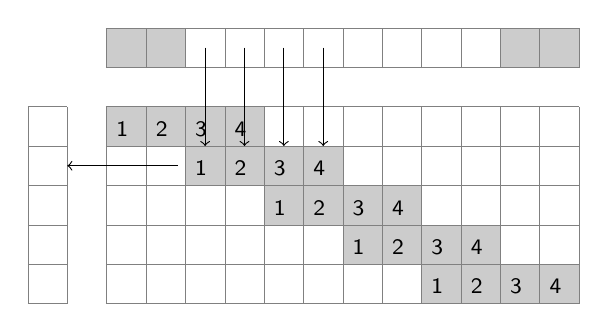
\begin{tikzpicture}[font=\footnotesize\sffamily]
        \fill[black!20!white] (1,3) rectangle (2,3.5);
        \fill[black!20!white] (6,3) rectangle (7,3.5);

        \foreach \x/\y in {0/0, 1/0.5, 2/1, 3/1.5, 4/2}
        {
            \fill[black!20!white] (\x + 1, 2.0 - \y) rectangle (\x + 3, 2.5 - \y);
            \node[above right] at (\x + 1.0, 2 - \y) {1};
            \node[above right] at (\x + 1.5, 2 - \y) {2};
            \node[above right] at (\x + 2.0, 2 - \y) {3};
            \node[above right] at (\x + 2.5, 2 - \y) {4};
        }

        \draw[step=0.5cm,gray,very thin] (0,0) grid (0.5,2.5);
        \draw[step=0.5cm,gray,very thin] (0.99,2.99) grid (7,3.5);
        \draw[step=0.5cm,gray,very thin] (0.99,0) grid (7,2.5);
        \draw [->] (2.25,3.25) -- (2.25,2);
        \draw [->] (2.75,3.25) -- (2.75,2);
        \draw [->] (3.25,3.25) -- (3.25,2);
        \draw [->] (3.75,3.25) -- (3.75,2);
        \draw [->] (1.9,1.75) -- (0.5,1.75);
    \end{tikzpicture}
    \caption{Convolution with stride 2 in 1D \citep{shi_is_2016}}
    \label{fig:1d_deconv}
\end{figure}
For images the output size of a deconvolutional (deconv) layer is calculated with the inverse formula for the output size of a convolutional layer. The stride defines the upsampling factor of this layer, the kernel size the ratio of 'overlapiness' and the padding is set accordingly.

\subsection{Fully convolutional network} % (fold)
\label{sub:conepts:fcn:fcn}
Proposed by \citet{long_fully_2015} \glspl{fcn} are a specific architecture of CNNs. Fully convolutional states that the network consists only of convolutional layers. As these are translation invariant the networks can take arbitrarily sized inputs and produce a coarse output.\\
The original authors use this architecture for semantic segmentation which means to assign each pixel in an image a semantic label (dog, person, tree, etc.). They build their network from classic semantic object classifiers like VGG-16 \citep{simonyan_very_2014}. These take fixed sized images as inputs and produce a single label thereby classifying the whole image. Typically these networks produce high level features through a series of convolutional layers and classify them with a single or a series of fully connected layers (inner product of the inputs). To label an image pixel-wise with such an architecture we would have to forward the neighborhood of each pixel through the network which would introduce an \bigO{w * h} time complexity ($w$ and $h$ being the width and the height of the image).\\
The fully connected layers can be directly converted to convolutional ones.
 These networks (as e.g. ) take full images as input then apply multiple convolutions and in the end classify the whole image with multiple fully connected layers which returns a class prediction vector over the trained classes. Viewing these fully connected layers as convolutions with kernels spanning the whole size of the layers input transforms them in convolutional layers and therefore the whole network into a \gls{fcn}. As the output of this network now will be a small grid of predictions the classification results have to be upsampled to the size of the input which can be done within the network by using deconv layers. Now we have a network which can predict and segment pixelwise in arbitrarily sized inputs and is end-to-end trainable.

\section{Residual Networks}
\label{sec:concepts:resnet}
After the succes of AlexNet \citep{krizhevsky_imagenet_2012}
